\documentclass[logo,reportComp]{thesis}
\usepackage[cpp,pseudo]{mypackage}

\title{自然语言处理}
\subtitle{作业一:中文分词}
\school{数据科学与计算机学院}
\author{陈鸿峥}
\classname{17大数据与人工智能}
\stunum{17341015}
\headercontext{自然语言处理作业}
\lstset{language=python}

\begin{document}

\maketitle

在本实验中我采用了三个分词工具对新华网\footnote{\url{http://www.xinhuanet.com/politics/leaders/2019-09/21/c_1125023359.htm}}的语料进行中文分词。
其中三个工具说明如下:
\begin{itemize}
	\item 北大分词(PKUSEG)\cite{bib:pkuseg}:北大基于之前发表的两篇ACL顶会论文整理出来的工具包,今年初才刚刚发布出来,宣称具有最高的准确率
	\item 结巴分词(jieba)\cite{bib:jieba}:号称要做最好的中文分词工具,也是最多人使用的开源中文分词工具包
	\item 清华分词(THULAC)\cite{bib:thulac}:清华大学自然语言处理与社会人文计算实验室研制推出的一套中文词法分析工具包
\end{itemize}

我编写了一段Python脚本,从文本中读入语料,并进行分词并输出,程序如下。
\begin{lstlisting}
import time
import pkuseg
import jieba
import thulac

with open("input.txt","r") as infile:
	intext = infile.read()
	# pkuseg
	print("Begin pkuseg...")
	seg = pkuseg.pkuseg()
	start = time.time()
	text = seg.cut(intext)
	end = time.time()
	res = "|".join(text)
	outfile = open("output_pkuseg.txt","w")
	outfile.write(res)
	print("Time (pkuseg): {:.4f}s".format(end-start),end="\n\n")

	# jieba
	print("Begin jieba...")
	start = time.time()
	text = jieba.cut(intext)
	end = time.time()
	res = "|".join(text)
	outfile = open("output_jieba.txt","w")
	outfile.write(res)
	print("Time (jieba): {:.4f}s".format(end-start),end="\n\n")

	# thulac
	print("Begin thulac...")
	thu = thulac.thulac(seg_only=True)
	start = time.time()
	text = thu.cut(intext)
	end = time.time()
	text = [t[0] for t in text]
	res = "|".join(text)
	outfile = open("output_thulac.txt","w")
	outfile.write(res)
	print("Time (thulac): {:.4f}s".format(end-start),end="\n\n")
\end{lstlisting}

运行过程与时间如下图所示。
\begin{figure}[H]
\centering
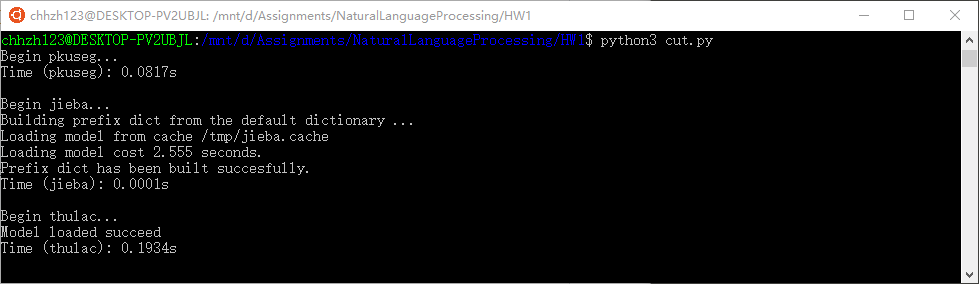
\includegraphics[width=\linewidth]{runtime.png}
\end{figure}
可以看到结巴分词的速度最快,北大的工具包次之,清华的最慢。

我采用了Sublime Text的工具包Sublimerge来对比不同工具输出的分词,如下图所示。
\begin{figure}[H]
\centering
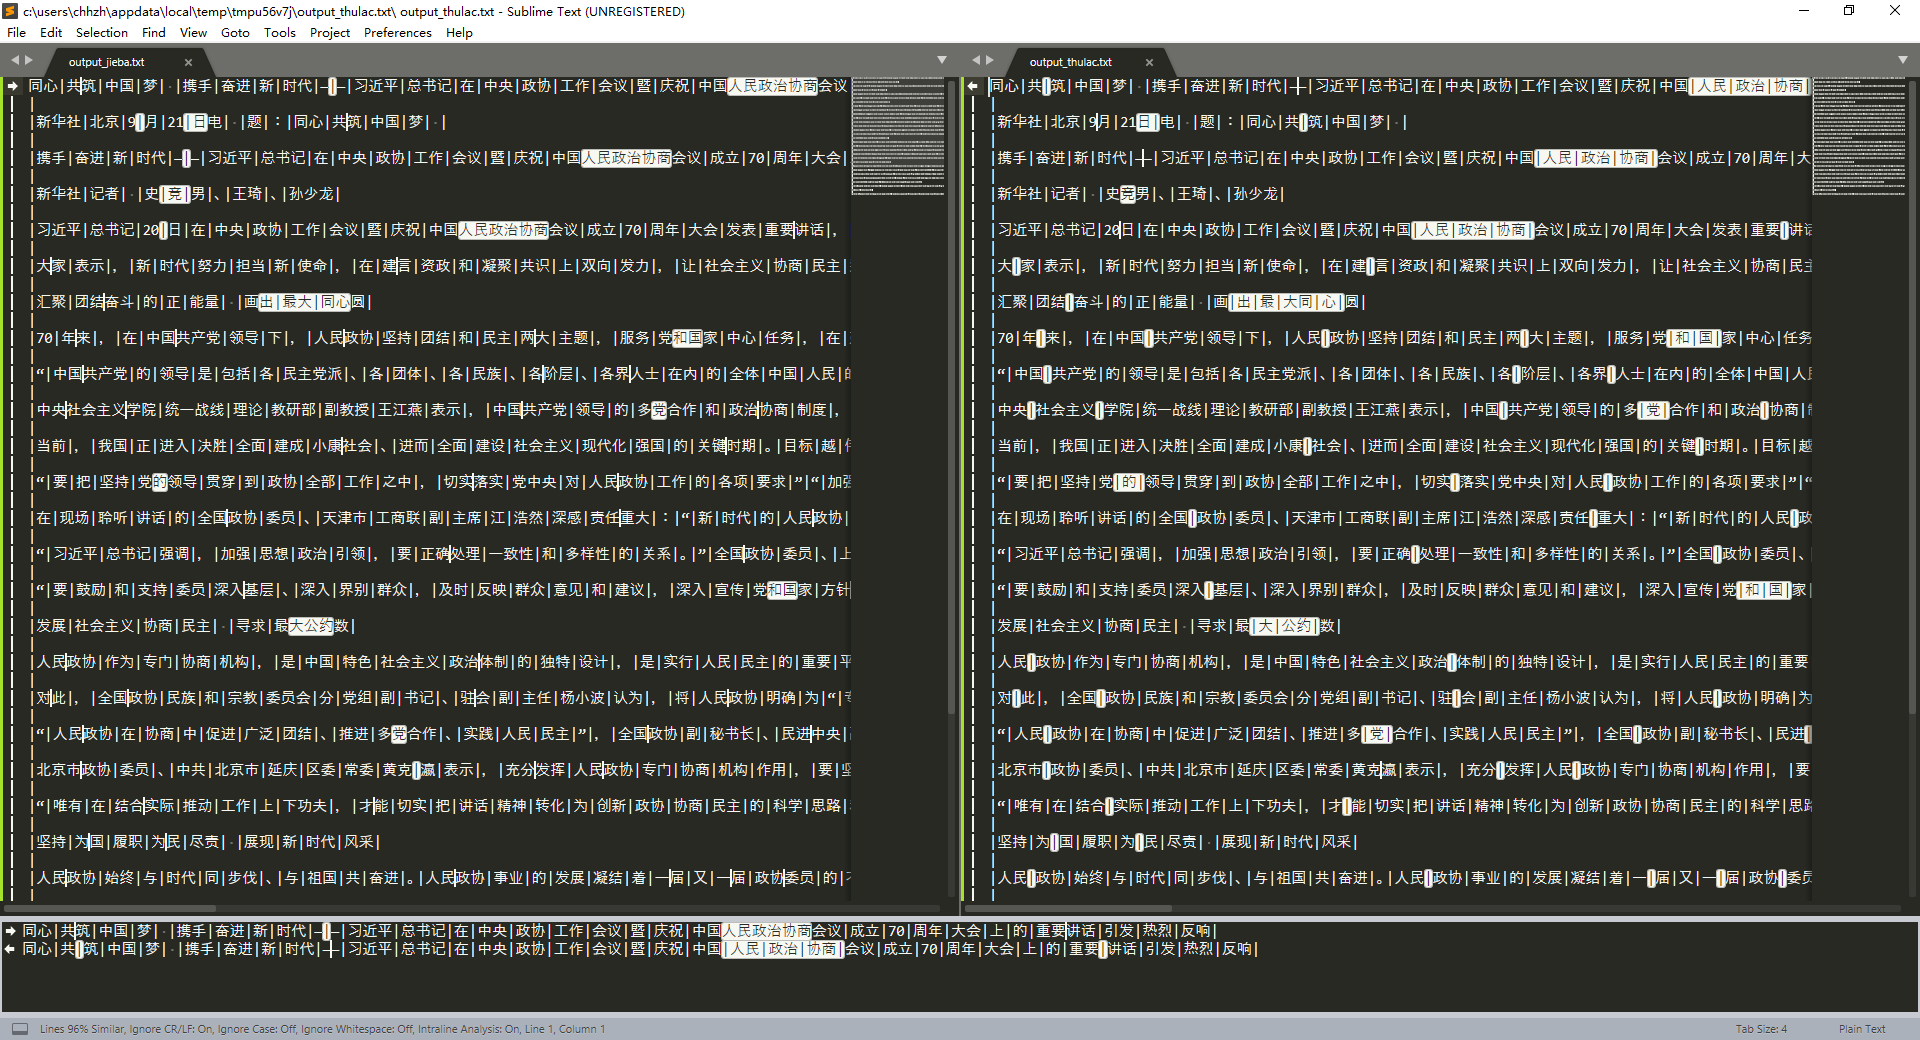
\includegraphics[width=\linewidth]{compare.png}
\end{figure}

通过分析,可以发现很多问题
\begin{itemize}
	\item 分词的粒度:清华的工具包可能没有专门针对新闻语料进行训练,因此会出现比较明显的问题,如下面第一条,清华工具包的断句明显是错的,它将\textbf{大同}连了起来,而没有辨别出\textbf{同心圆}。而且在可断可不断的点,清华工具包更倾向于断,如下表的后三条语料。
	从下面几个例子来看,结巴分词对于词语长度的掌握在几种工具中比较好。
	\begin{center}
	\begin{tabular}{cccc}\hline
	原始语料 & PKUSEG & Jieba & THULAC\\\hline
	画出最大同心圆 & 画出$\mid$最$\mid$大$\mid$同心圆 & 画出$\mid$最大$\mid$同心圆 & 画$\mid$出$\mid$最$\mid$大同$\mid$心$\mid$圆\\
	来自不同方面 & 来自$\mid$不同$\mid$方面 & 来自$\mid$不同$\mid$方面 & 来$\mid$自$\mid$不$\mid$同$\mid$方面\\
	中国民间文艺家协会 & 中国$\mid$民间$\mid$文艺家$\mid$协会  & 中国民间文艺家协会 & 中国$\mid$民间$\mid$文艺$\mid$家$\mid$协会\\
	最大公约数 & 最$\mid$大$\mid$公约数 & 最大公约数 & 最$\mid$大$\mid$公约$\mid$数\\
	\hline
	\end{tabular}
	\end{center}
	\item 对于人名等专有名词的辨别:这也是我这次实验中比较关注的点,会发现这些分词工具对于人名的辨别还是比较差的,经常需要附加的标点符号或标志词(如“说”)来进行辨别。
	而在这一点上,结巴分词就做得比较糟糕了,经常辨别不出人名,如下面的例子,常常将人名中的名字部分分开。
	而且三个分词软件都不能很好辨别\textbf{江浩然}这一人名,因为在大部分语料中,浩然是自成一词,而这些模型都没有足够的具体情况具体分析的能力,故都会选择断开。
	\begin{center}
	\begin{tabular}{cccc}\hline
	原始语料 & PKUSEG & Jieba & THULAC\\\hline
	史竞男 & 史$\mid$竞男 & 史$\mid$竞$\mid$男 & 史竞男\\
	黄克瀛 & 黄克瀛 & 黄克$\mid$瀛 & 黄克瀛\\
	江浩然 & 江$\mid$浩然 & 江$\mid$浩然 & 江$\mid$浩然\\
	\hline
	\end{tabular}
	\end{center}
	\item 不同语料训练出来的模型:这里主要看PKUSEG提供的不同预训练模型。
\begin{figure}[H]
\centering
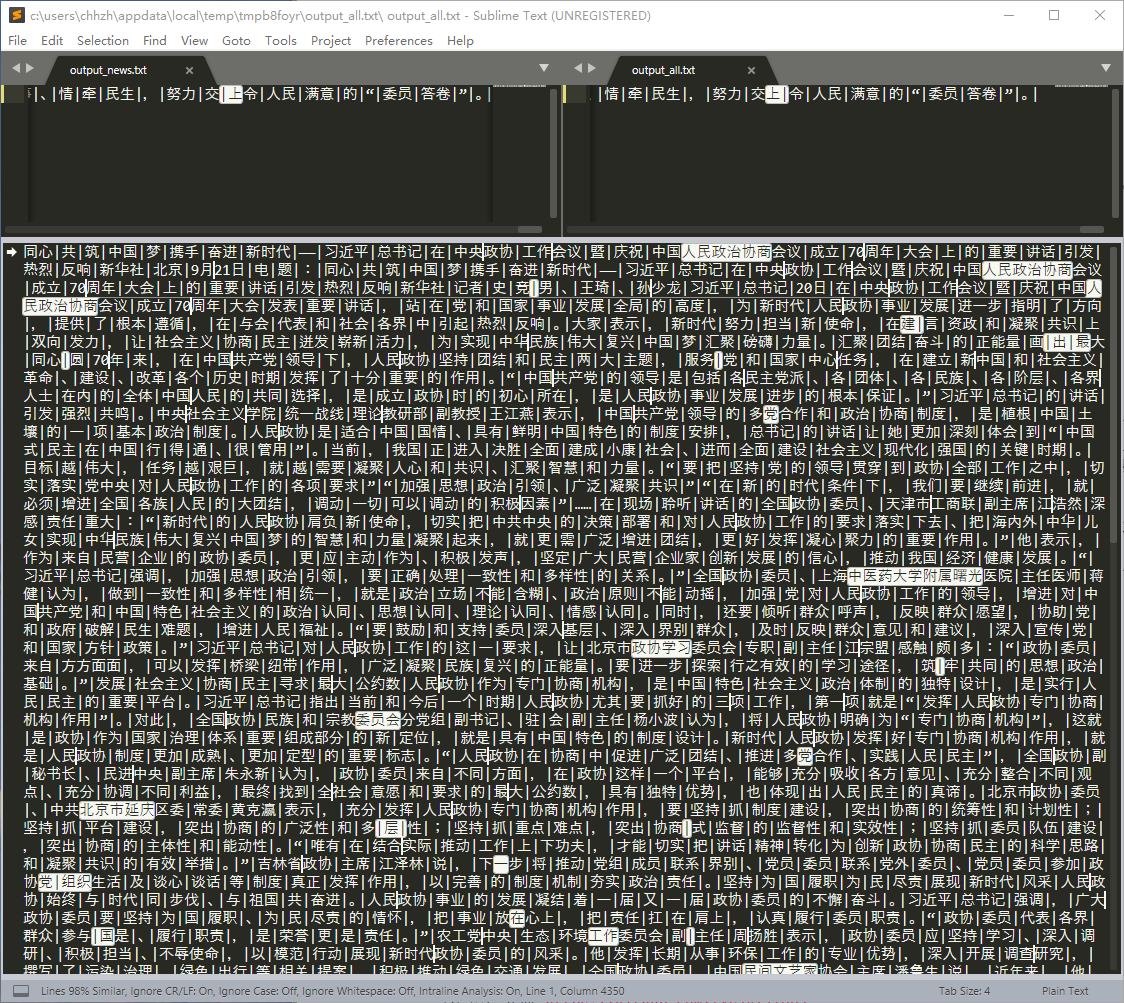
\includegraphics[width=\linewidth]{compare2.png}
\end{figure}
	可以看到,用新闻语料预训练出来的模型分词粒度会比较大,能够很好地辨别专有名词,而混杂语料训练出来的模型则倾向于细粒度的划分。具体的例子包括\textbf{中国人民政治协商会议}、\textbf{中国民间文艺家协会}、\textbf{上海中医药大学附属曙光医院}等,这些新闻语料预训练模型都能将其当成一个整体看待。
\end{itemize}

所有的程序及输出文件都附在附件中,可以进行查看。

\begin{thebibliography}{99}
\bibitem{bib:pkuseg} Ruixuan Luo, Jingjing Xu, Yi Zhang, Xuancheng Ren, Xu Sun. PKUSEG: A Toolkit for Multi-Domain Chinese Word Segmentation. Arxiv. 2019. \url{https://github.com/lancopku/PKUSeg-python}
\bibitem{bib:jieba} 结巴分词, \url{https://github.com/fxsjy/jieba}
\bibitem{bib:thulac} 孙茂松, 陈新雄, 张开旭, 郭志芃, 刘知远. THULAC:一个高效的中文词法分析工具包. 2016. \url{https://github.com/thunlp/THULAC-Python}
\end{thebibliography}

\end{document}

% ❑ 注意事项:
% 1) 可以调用任何中文分词工具;
% 2) 词语之间用“|”分割;
% 3) 列举、归纳碰到的问题;
% 4) 把结果发到邮箱: wangjh237@mail2.sysu.edu.cn
% 邮件主题: 《自然语言处理》 中文分词作业+(姓名,学号)
% 例如: 《自然语言处理》 中文分词作业(张三, 201984541)